%
% File acl2019.tex
%
%% Based on the style files for ACL 2018, NAACL 2018/19, which were
%% Based on the style files for ACL-2015, with some improvements
%%  taken from the NAACL-2016 style
%% Based on the style files for ACL-2014, which were, in turn,
%% based on ACL-2013, ACL-2012, ACL-2011, ACL-2010, ACL-IJCNLP-2009,
%% EACL-2009, IJCNLP-2008...
%% Based on the style files for EACL 2006 by 
%%e.agirre@ehu.es or Sergi.Balari@uab.es
%% and that of ACL 08 by Joakim Nivre and Noah Smith

\documentclass[11pt,a4paper]{article}
\usepackage{acl2019}
\usepackage{times}
\usepackage{latexsym}
\usepackage{graphicx}
\usepackage{hyperref}
\usepackage{float}
\usepackage{url}

\aclfinalcopy % Uncomment this line for the final submission 
% \def\aclpaperid{***} %  Enter the acl Paper ID here

\setlength\titlebox{4cm}  
% You can expand the titlebox if you need extra space
% to show all the authors. Please do not make the titlebox
% smaller than 5cm (the original size); we will check this
% in the camera-ready version and ask you to change it back.

\title{Imperial College: `Don't Patronize Me!' Coursework 2024}

\author{Anton Zhitomirsky \\
  Imperial College London \\
  \texttt{az620@ic.ac.uk} \\
  \href{https://gitlab.doc.ic.ac.uk/az620/nlp-cw-2024}{\texttt{gitlab.doc.ic.ac.uk/az620/nlp-cw-2024}} \\
  hash: 01b67724bcf0d6d22a859fcdc37f4fcb7f32e77a \\ 
}

\begin{document}
\maketitle

\section{Introduction}

% \textbf{5 marks}: Introduction, with an explanation of the task and the
% dataset. You may want to read/cite the task paper (and any other paper of
% your choosing).

Most social media websites contain portals through which even unregistered users can view their content. Focusing primarily on textual posts, this leaves many vulnerable users to unfiltered content, which may be harmful if not regulated. \citet{Ng-discrimination} concludes that regardless of intention, if this content goes unfiltered it may ``justify'', ``encode'', ``enact'' and ``routinize'' discrimination amongst targeted groups.

This motivates the creation and popularization of The Don't Patronize Me! dataset to provide a source for engineers to develop categorization algorithms to progress the protection of targeted groups. The dataset, authored by \citet{perez-almendros-etal-2020-dont}, is a labelled dataset containing more than 10,000 paragraphs extracted from news stories, country of origin, and keyword which is then labelled indicating its level of Patronizing and Condescending Language (PCL).

I propose an extension to the base-line categorization model `\texttt{RoBERTa}' which beats the initial benchmarks of \texttt{0.48} F1-score on the dev-set and \texttt{0.49} on the test-set. The repository link is available at the top of this report.

\begin{table}[!h]
    \centering
    \begin{tabular}{|l||c|c|}
        \hline
         & F1 dev-set & F1 val-set \\
        \hline
        \hline
        Baseline Model & 0.48 & 0.49 \\
        \hline
        Proposed Model  & 0.82 & 0.57 \\
        \hline
    \end{tabular}
    \caption{F1 score of PCL language for baseline model compared to final model}    
\end{table}

\section{Data Analysis}

% \emph{For a written description of the training data. This should include}

% \begin{enumerate}
%     \item \textbf{5 marks}: Analysis of the class labels: how frequent these are and how they correlate with any feature of the data, e.g. input length.
%     \item \textbf{10 marks}: Qualitative assessment of the dataset, considering either how hard or how subjective the task is, providing examples in your report.
% \end{enumerate}

\subsection{Feature Distribution}\label{sect:feature-distribution}

Labels arrive annotated by two main annotators. Their values span from $[0,4]$ indicating the level of PCL within the text snippet. \citet{perez-almendros-etal-2020-dont} explains how both annotators individually classify each sentence with a score in the range $[0,2]$ to indicate the strength of PCL from: no PCL, borderline PCL and blatant PCL. These scores were then summed to produce a 5-point scale of PCL, where the range $[0,1]$ indicates a negative example, and $[2,4]$ indicating a positive example.

Data also arrives with labeled country information indicating the source media outlet, and a keyword field. The keyword is provided as input to the model as the search term used to retrieve texts about a target community. A distribution of these fields is shown in Figure~\ref{fig:dev-set-distribution}. Here, the supplied dev dataset contains a disproportionate number of negative (9475) and positive (993) examples of PCL.

\begin{figure*}[h!]
    \centering
    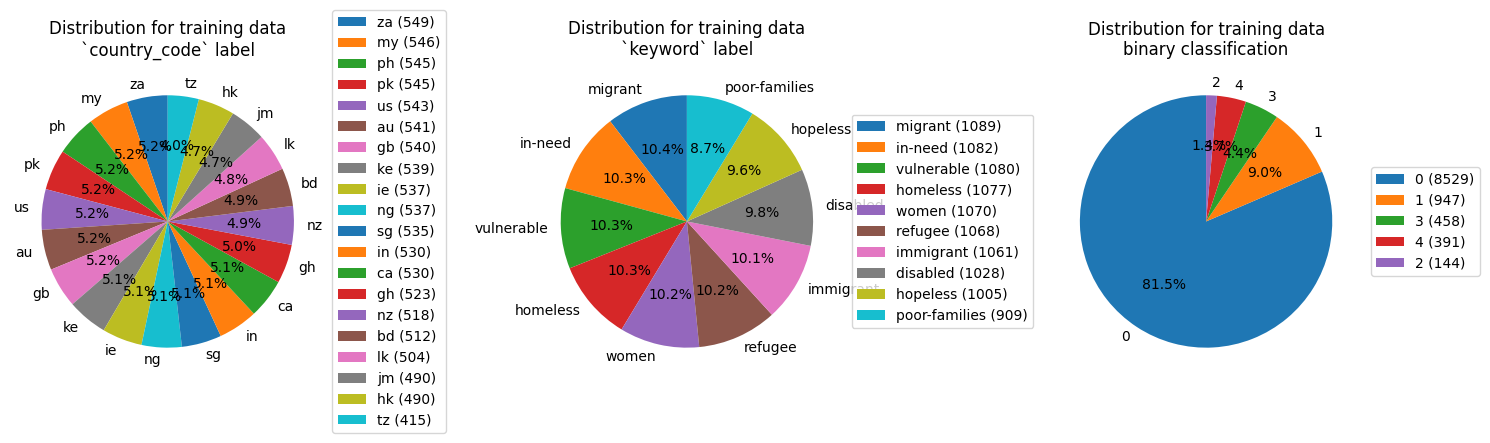
\includegraphics[trim=0cm 0cm 0cm 0cm, clip, width=\linewidth]{figures/test_distribution.png}
    \caption{Pie charts of different label distributions in the supplied dev-set}
    \label{fig:dev-set-distribution}
\end{figure*}

\begin{figure}[H]
    \centering
    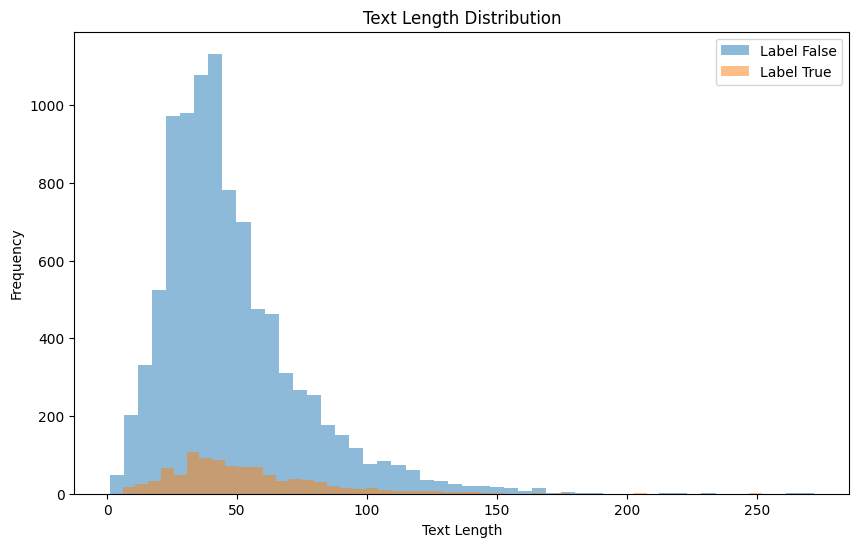
\includegraphics[trim=0cm 0cm 0cm .8cm, clip, width=\linewidth]{figures/text-input-length-by-binary-patronizing.png}
    \caption{Histogram of word count by PCL (true) and non PCL (false)\footnotemark}
    \label{fig:word-count}
\end{figure}

\footnotetext{Without loss of generality, text with more than 250 words have been clipped}

Furthermore, the distribution of word counts between the two (See Figure~\ref{fig:word-count}) offers no obvious underlying pattern between the two classes. This was further supported by the unequal variances t-test which returned a p-value of $1.331 \times 10^{-7}$ which is not enough to reject the hypothesis that the means are the same. Therefore, there is no correlation between the length of the input and the PCL label.


\subsection{Subjective Difficulty}

Indeed, \citet{perez-almendros-etal-2020-dont} mention the subjective nature of the task as it is complicated. The word `lovely' appears uniquely in PCL text examples. This word isn't negative, but in the context of the sentence (par\_id: 2404) ``We think it's lovely that so many have come forward to help out a family clearly in need!'' the sentence has been labeled as blatantly PCL with a score of 3. In-fact, tweaking the sentence from ``a family clearly in need'' to ``families in need'' removes entitlement and converts it to compassion. However, this is once again subjective, depending on intonation and cadence.

\subsection{Artifacts}\label{sect:artifacts}

The flexible environment of news articles allows for authors to post resources and further reading, like in the case of par\_id: 2838: \emph{``Read more about the site's history here: [LINK]''}. Therefore, with a primitive language processing model, we cannot determine the degree of PCL from a link. Some links and references are also clipped in the source with token ``TOOLONG'' which also aught to be pre-processed to avoid confusion from the model. Additionally, writers are free to reference other users (par\_id: 5598 ``@toekunbore [...]''), the handle of which would likely be ignored by language models.

Lastly, adding to the complexity of processing language, we must also filter and process out-of-vocabulary words. This may appear in the form of a typo like in par\_id: 8221 \emph{``Do they think it is "" \textbf{jsutice} "" \textbf{ti} imprison [...]''}, hyperboles like par\_id: 5333 \emph{``But \textbf{nooooo} [...]''}, or slang like in par\_id: 1674 \emph{``Kyle really your a pig, \textbf{lol} [...]''}.

However, we cannot place too much focus on filtering typos, as this is a common technique employed by social media `trolls' to avoid automatic PCL detection; this is a cat-and-mouse game which even the most sophisticated language models employed by the largest companies cannot win. We will continue with the assumption that the data is mostly clean.

% \textbf{10 marks}: Further model improvements (beyond using a bigger transformer model), for example pre-processing, data sampling, data augmentation, ensembling, etc. Two main improvements, with a third less explored improvement is sufficient. For example: try several different data sampling approaches, try several data augmentation strategies by perturbing observations in different ways, and then see if incorporating one of the categorical columns improves performance.

% \begin{itemize}
%     \item try and balance out the classes by applying synonyms to low frequency labels
%     \item data-sampling, research: is it common to feed in an equal proportion of each class in batches during training?
%     \item using country code also
% \end{itemize}

\section{Preprocessing: Minority Upsampling}

The data is very imbalanced; Section~\ref{sect:feature-distribution} discusses the sparsity of positive PCL examples in the training data. Therefore, it is possible that the model may experience great performance in the majority negative class, and fail to learn details about the minority positive class (\citet{alberto-imbalanced-datasets}).

We can synthetically produce more data points for the minority positive class by changing the content of the sample without changing the sentiment of the text. 

\subsection{Failed Considerations}

Even the most popular augmentation techniques are task specific. These were considered, but ultimately not implemented.

\subsubsection{Stop Word Removal}

Stop words contain little value, so they can be useful to decrease the length of sentence. However, it may change the sentiment of a sentnece: ``I do not like you because I'm better than you'' changed into ``I like I'm better'' -- removing all PCL sentiment from the sentence -- and rendering an ineffective augmentation.

\subsubsection{Easy Data Augmentation}

\citet{wei-zou-2019-eda} propose a pipeline to tweak sentences by replacing, deleting, swapping and inserting words. The authors comment that by fine-tuning replacement parameters and the upsampling factor, it can ``can boost performance on text classification tasks''. However, we found that the model quickly overfit within one epoch.

\subsubsection{Rephrasing Models}

Further effots were dedicated to rephrasing the text with the help of a pre-trained GPT-2 model as suggested by \citet{Dai2023AugGPTLC}. However, significant inconsistencies were discovered depending on the sentence length, so ultimately this effort was abandoned.

\subsection{Successful Considerations}

\subsubsection{Translation}\label{sect:translation}

This upsampling technique is inspired by \citet{nlp-imbalanced-data} who suggests translating the text into a non-English language and then back into English. The hope is that translating back introduces new wording and structure without augmenting the sentiment of the sentence. We take this a step further by introducing a parameter to control the depth of translation.

\subsubsection{Swapping Sentences}

Within the same paragraph, we can swap the ordering of sentences. This augmentation was less researched but helped add variance to the upsampling the variance of the minority class.

\section{Data Augmentation}

\subsection{Tokenization}

By tokenizing the input, we can efficiently assign \texttt{[UNKNOWN]} tokens to out-of-vocabulary words. This is important for a pre-trained model which is trained on well-formed English text, and may not understand slang or typos.

\subsection{Masking inputs}

Further benefit of tokenization includes the choice of randomly masking a subset of words in the input. This allows models to capture rich contextual information and dependencies in language. This means that our model generalizes well to various text classification tasks, even when faced with different writing styles, vocabulary, and sentence structures, which is vital for detecting unseen ways to patronize.

\section{Model}\label{sect:model}

\subsection{Final model predictions}

Experiments were conducted on BERT, RoBERTa, and DistilBERT architectures. RoBERTa performed the best, and therefore was used as the base model for the final architecture. We considered masked and un-masked models, and found that the masked model performed better. The results are shown in Table~\ref{tab:final-model-predictions}.

\begin{table*}[!h]
    \centering
    \begin{tabular}{|c||c|c|c|c|}
        \hline
        Model & \multicolumn{2}{|c|}{Masked} & \multicolumn{2}{c|}{Un-Masked} \\
         & F1 dev-set & F1 val-set & F1 dev-set & F1 val-set \\
        \hline
        \hline
        BERT uncased & - & - & 0.86 & 0.5363 \\
        BERT cased & - & - & 0.9465 & 0.5097 \\
        RoBERTa & 0.8193 & \framebox{0.5727} & 0.8677 & 0.5404 \\
        DistilBERT & 0.7989 & 0.5152 & 0.8007 & 0.4949 \\
        \hline
    \end{tabular}
    \caption{F1 score of PCL language models attempted}    
    \label{tab:final-model-predictions}
\end{table*}

\subsection{Hyper-parameters}

\begin{table}[H]
    \centering
    \begin{tabular}{|c|c|}
        \hline
        hyper-param & value \\
        \hline
        \hline
        text truncation & 300 \\
        mask tokens & True \\
        mlm probability & 0.15 \\
        batch size & 16 \\
        learning rate & $2 \times 10^{-5}$ \\
        epochs & 5 \\
        warmup steps & 100 \\
        weight decay & 0.01 \\
        weighted loss & True \\
        translation depth & 3 \\
        \hline
    \end{tabular}
    \caption{Hyper-parameters}
    \label{tab:hyper-parameters}
\end{table}

For the final model architecture, we use a linear layer on top of a RoBERTa base model. The submission model has 2 output neurons, corresponding to non-PCL and PCL -- the higher neuron is the prediction. We trained the model for 5 epochs with no early stopping and an initial learning rate of $2 \times 10^{-5}$. Even through the different BERT flavours have similar performance -- which we hypothesize is due to the data augmentation step -- we chose the best performance on a validation set (see Table~\ref{tab:final-model-predictions}).

The most significant model improvement was the introduction of a weighted loss criterion, which scales loss depending on the rarity of the class in the dataset. In this case, the loss is scaled significantly for PCL examples, of which there are few. This means that the model is incentivized to learn information from the minority class.

\section{Results}

\subsection{Comparison}

We implemented 2 simple models based on a Bag of Words approach. After segmenting all input sentences by spaces and finding unique `words' (some of which are strings of punctuation), we encode the number of occurences of each word in the vocabulary per document in the corpus. On this matrix, we then fit a Gaussian Naive Bayes model and a Logistic Regression model. The models got positive class F1 scores of $0.14$ and $0.28$ on test data, respectively.

The highest weighted words in the Linear Regression model, that is, the words whose appearance most strongly correlates with PCL are: \texttt{'burlesque', 'duty', 'Dreamers', 'hearts', 'Christmas'}. An example sentence in which one of these words appears is: \emph{``Dreamers are immigrants who were brought into the United States illegally as children . Under the program President Obama created , " Dreamers " have been allowed to stay legally''}. It is very likely that the model overfits, and because of the model, it is unable to learn the true context of the word.

\section{Analysis}

\subsection*{Effect of level of PCL on model performance}

\begin{figure}[H]
    \centering
    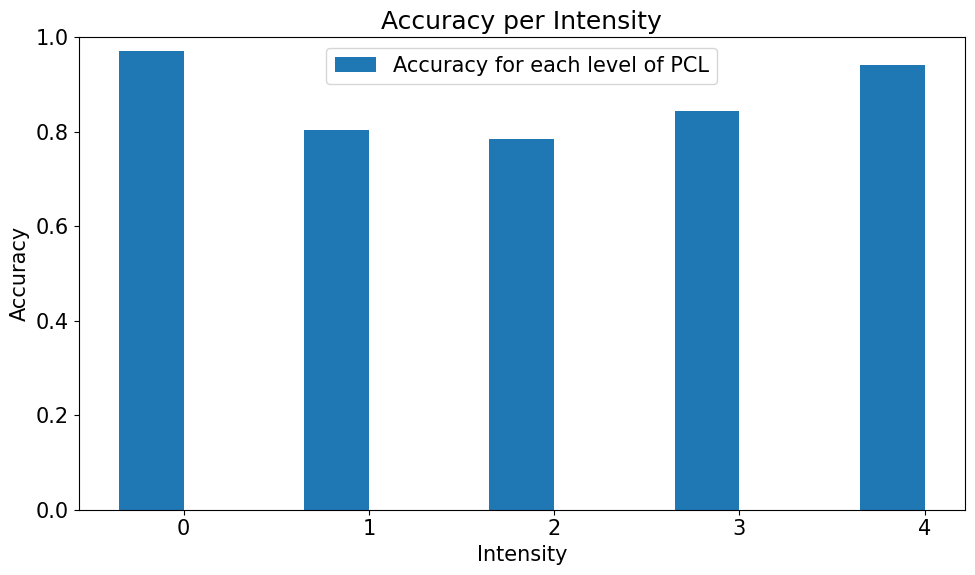
\includegraphics[width=\linewidth]{figures/accuracy_per_pecl_lebl.png}
    \caption{Accuracy of each PCL category}
    \label{fig:accuracy-per-pcl-cateogry}
\end{figure}

Figure~\ref{fig:accuracy-per-pcl-cateogry} shows that the model is the best at categorizing the two extremes of PCL, and is worse at categorizing the middle categories. This is likely because these are the most subjective; indeed, we recall from \citet{perez-almendros-etal-2020-dont} that labels between 1 and 3 are the texts which contain the most clashing options between annotators on the binary scale (where, for instance, a score of 1 is because one annotator scored 0 and the other 1).

We therefore conclude that the model is as good at categorizing the blatant PCL as it is for obvious non-PCL, with the least accuracy in the boundary labels between label 1 and label 2.

\subsection*{Effect of input sequence length on model performance}

\begin{figure}[H]
    \centering
    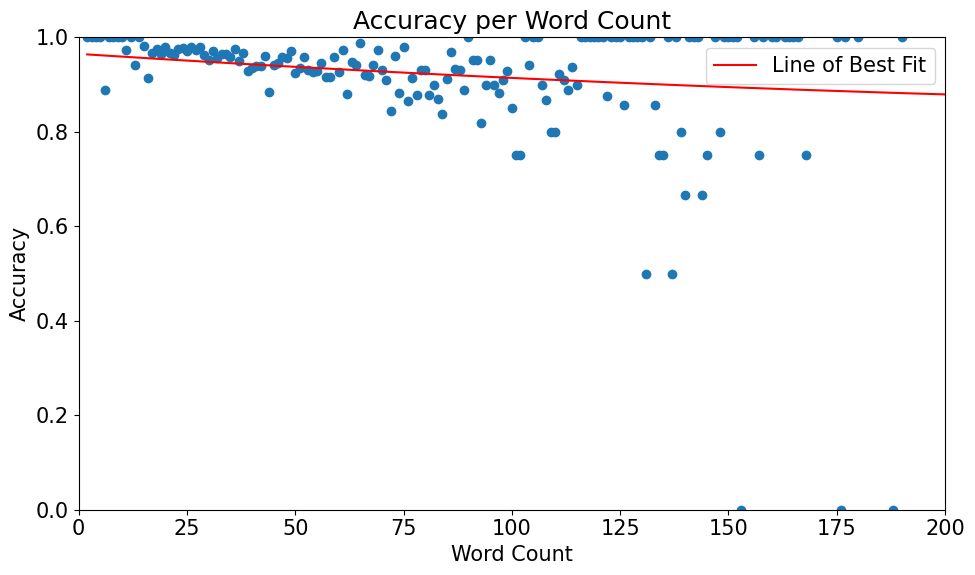
\includegraphics[width=\linewidth]{figures/accuracy_due_to_word_length.png}
    \caption{Accuracy of model against word count}
    \label{fig:accuracy-word-count}
\end{figure}

Figure~\ref{fig:accuracy-word-count} shows that the overall accuracy of the model declines as we increase the word count. We note that for sentences greater than $300$ this is likely to converge, as the tokenizer used truncates sentences to this length. However, the overall downward trend is likley due to attention in the RoBERTa model architecture. As the word count grows, the model's ability to capture and process dependencies between distant words may diminish, leading to a decline in overall accuracy.

\subsection*{Effect of PCL category on model performance}

\begin{figure}[H]
    \centering
    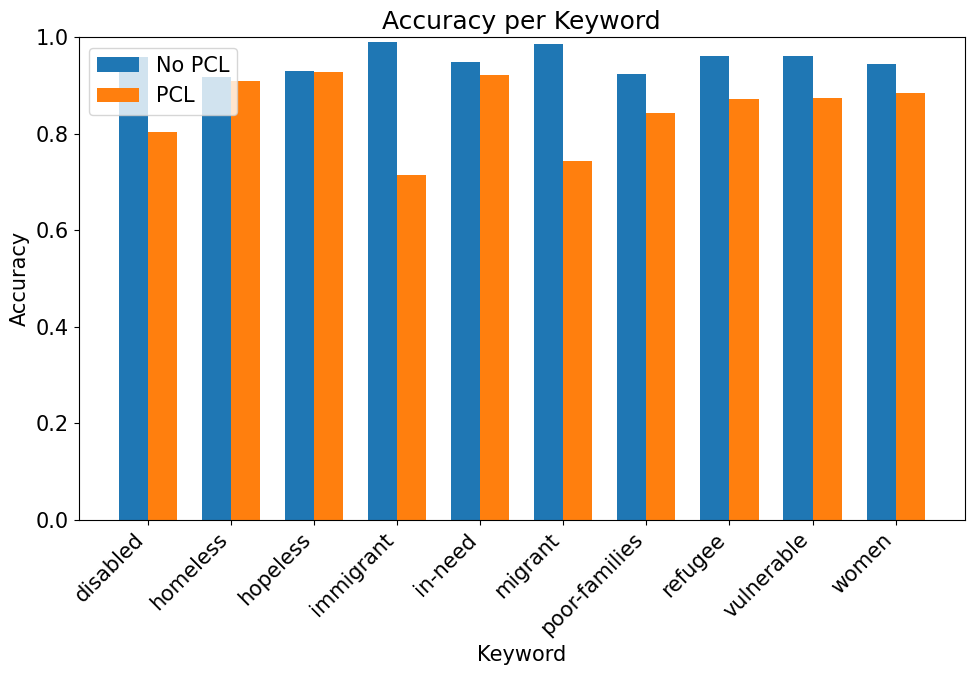
\includegraphics[width=\linewidth]{figures/accuracy_per_pcl_type_keyword.png}
    \caption{Accuracy of model against keyword of targeted group}
    \label{fig:accuracy-keyword}
\end{figure}


The keyword was not used during trianing, and therefore, the model lacks context regarding the background of the text. It therefore is left to find the abstract themes itself. Figure~\ref{fig:accuracy-keyword} shows this, and an especially poor accuracy for keyword:`immigrant' and `migrant'. These keywords are related, and the model is inaccurate when classifying whether there's PCL in text for these two classes. Conversely, the accuracy of non-PCL language for these keywords is very high, suggesting that the model is is likely to predict non-PCL language for these keywords.

\section{Conclusion}

In conclusion, the combination of careful pre-processing and data augmentation techniques with masking and a fine-tuning has outperformed the baseline model with an F-1 score of 0.82 and 0.57 for the train and validation set respectively. We have also shown that the model is better at predicting extremes of patronizing content, but less accurate for borderline cases: where the distinction between non-PCL and PCL becomes more subjective. 

An important finding from the analysis is that the model is not as accurate when classifying PCL language for the keywords `immigrant' and `migrant'. It is however very good at predicting whether sentences do not contain PCL -- this is wanted behaviour. If the model were to be deployed on a social media platform, it would be very unlikely to censor non-PCL language.

Further research should be made to encode information regarding the available `keyword' field into the model to provide a better theme encoding to influence the PCL categorization. Additionally, the model should be tested on a more balanced dataset, as this is very likely to improve test performance. Finally, it was hypothesized that typos in the model, as mentioned in Section~\ref{sect:artifacts}, would be ignored during the tokenizer stage, which could allow users to bypass the model. An improvement would be to come up with novel ways to manage typos, and possibly, intentional encodings (such as `leetspeak' and `pig latin').

\bibliography{references}
\bibliographystyle{acl_natbib}

\appendix

\section{Supplementary Material}

\begin{figure}[H]
    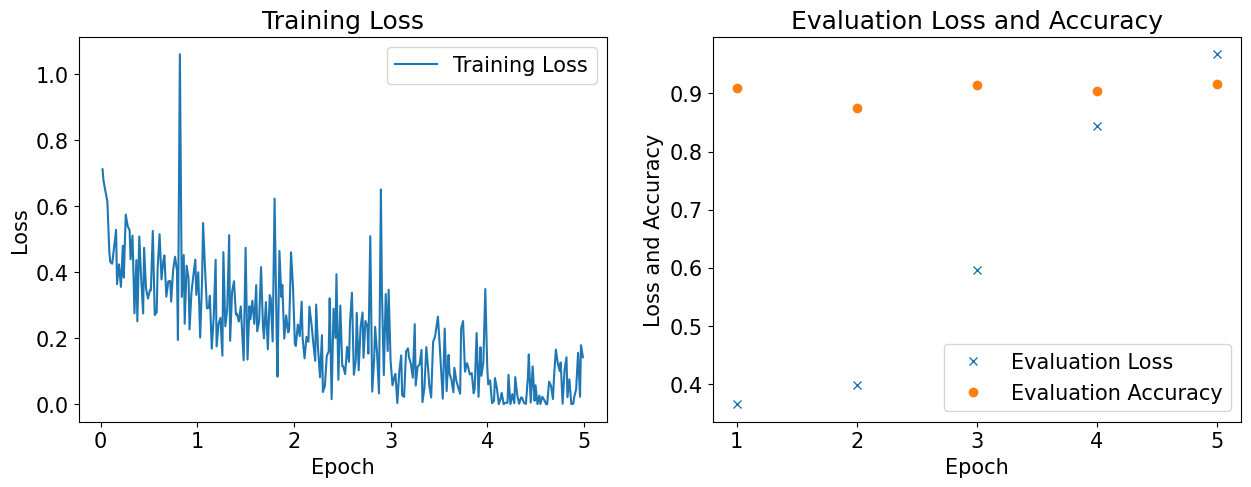
\includegraphics[trim=0 0 15.5cm 0, clip, width=\linewidth]{figures/final-loss.png}
    \caption{Training loss for the final submission model}
    \label{fig:final-loss}
\end{figure}

\end{document}
